\documentclass[12pt]{elsarticle}

\usepackage{lineno,hyperref,notoccite,etoolbox}
\makeatletter
\def\ps@pprintTitle{%
	\let\@oddhead\@empty
	\let\@evenhead\@empty
	\def\@oddfoot{\centerline{\thepage}}%
	\let\@evenfoot\@oddfoot}
\makeatother
\usepackage{setspace}
\singlespacing
\usepackage{mathptmx}
\usepackage{float,wrapfig}
\usepackage[margin=1in]{geometry}
\usepackage{booktabs}
\usepackage{cancel}
\usepackage[fleqn]{amsmath}
\usepackage{amssymb}
\allowdisplaybreaks
\newcommand{\bnumbers}{\begin{enumerate}}
	\newcommand{\enumbers}{\end{enumerate}}
\newcommand{\vs}{\vspace{2mm}}
\newcommand{\beq}{\begin{equation*}}
\newcommand{\eeq}{\end{equation*}}
\newcommand{\rr}[1]{\mbox{#1}}
\newcommand{\longequals}{{=\joinrel=}}
\newcommand{\squared}{$^{2}$}
\newcommand{\subtwo}{$_{2}$}
%tables
\setlength{\arrayrulewidth}{0.5mm}
\setlength{\tabcolsep}{5pt}
\renewcommand{\arraystretch}{1.75}
\newcommand{\fullline}{\noindent\rule{14cm}{0.4pt} \vspace{4mm}}
\usepackage{subfigure}


\begin{document}
\begin{flushright}
	Ember Sikorski\par
	Final\par
	ECE 624\par 
	10 December 2018
\end{flushright}


\begin{enumerate}
%1	
\item Discuss why space charge limited conduction could occur in a device comprised of an
a-semiconductor. Use energy band diagrams in your discussion. 
\par 
\fullline

%2
\item The UV-Vis transmission data is shwon for several a-semiconductor films in \textbf{Fig. 1}. Based on the optical data, what can you say about the effect of the particular dopant on the sample? Which sample would you expect to have the most defects? Describe why you support your conclusions.

\begin{figure}[H]
	\centering
	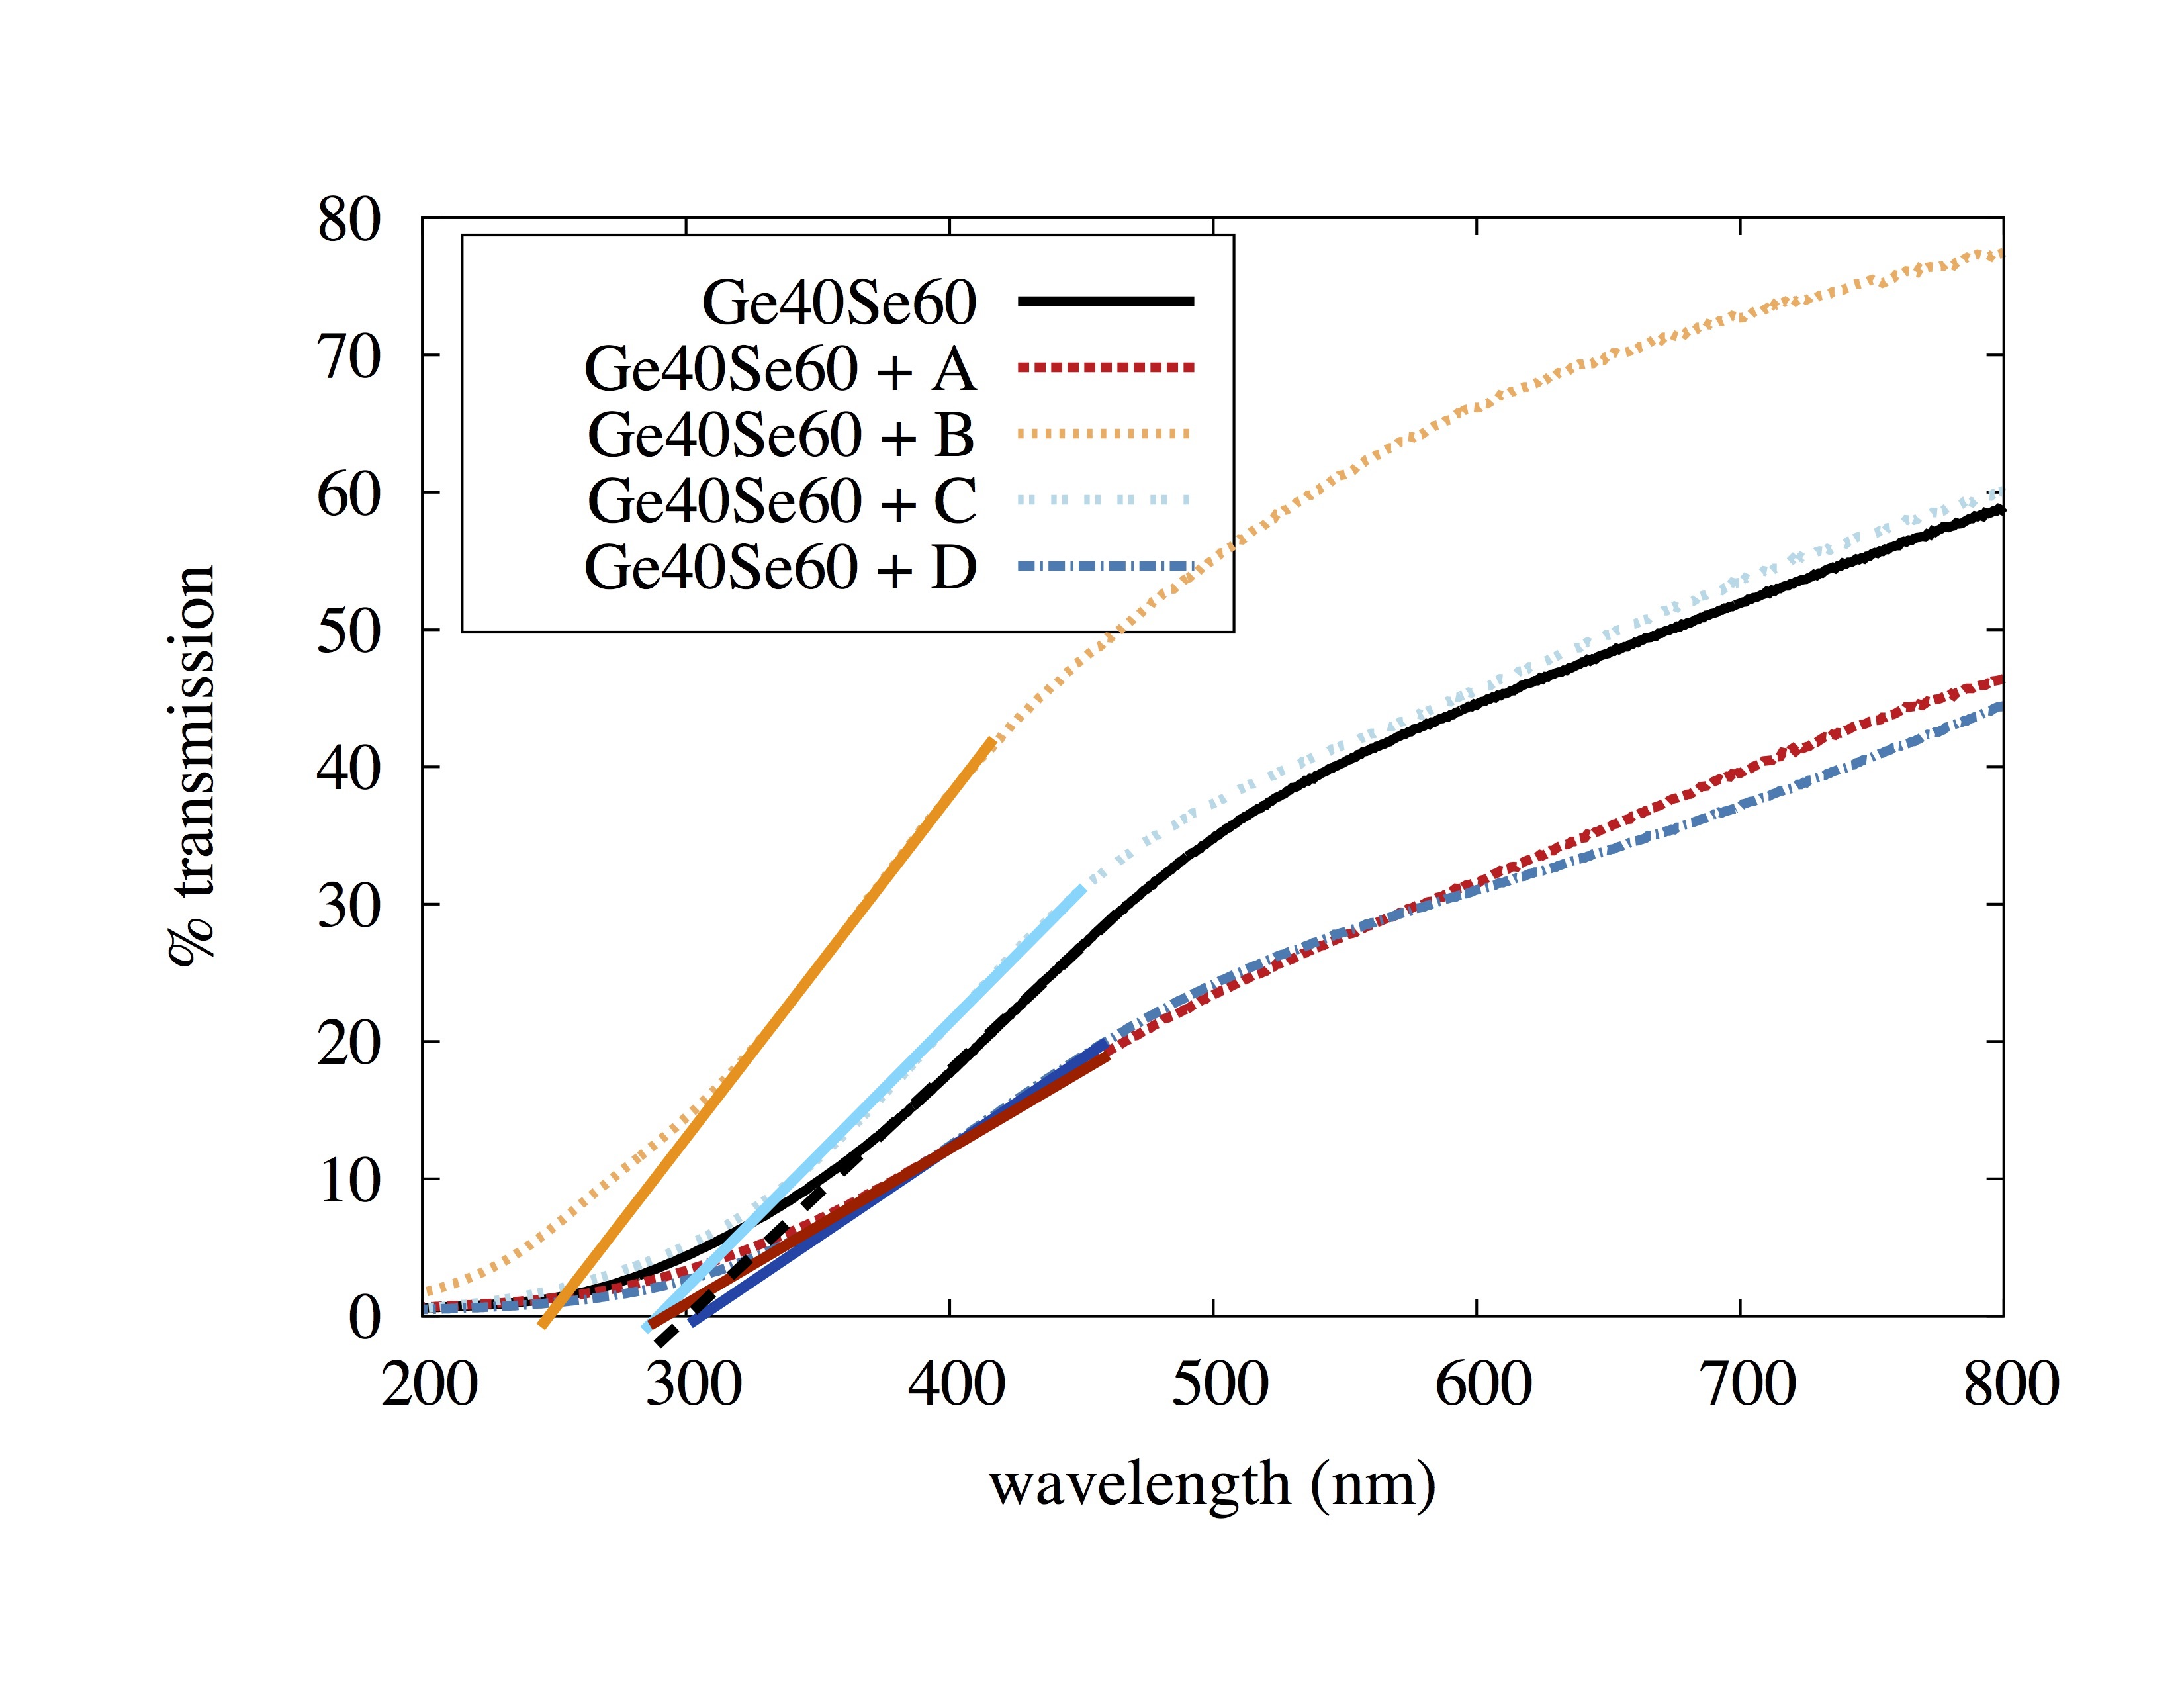
\includegraphics[width=0.6\textwidth]{fig1}
	\caption{UV-Vis \% transmission data for Ge$_{40}$Se$_{60}$ films.}
\end{figure}
\par 

The approximate optical bandgap is shown by taking the tangent of the linear portions of the optical data and finding the intercept at 0\% transmission. The original Ge$_{40}$Se$_{60}$ sample and those doped with A, C, and D give optical bandgaps around 300 nm or $\approx$ 4 eV ($\lambda=hc/E$), while Ge$_{40}$Se$_{60}$ + B has an optical bandgap of approximately 250 nm or $\approx$ 5 eV. While electrical conduction ideally requires transitions from the valence extended states to the conduction extended states, the optical band gap can include shorter transitions from the localized states in the gap to the conduction extended states. As seen in Raty et al.'s study of aging in phase change materials \cite{Raty2015}, a decrease in localized defect states leads to band gap widening. Of the four dopant samples, Ge$_{40}$Se$_{60}$ + D leads to the smallest optical band gap (<4 eV) and thus likely as the most defects.

\fullline

%3
\item Compare and contrast the derivation of the density of states for a crystalline
semiconductor with that of an amorphous semiconductor.
\par 
\fullline

%4 
\item Describe conduction in the extended states, band tail (mobility edge) states, and in the
gap states. 
\par 
\fullline

%5
\item Suppose you are going to make electrical measurements on an a-semiconductor. How
would you do this to ensure you could differentiate between contributions to current due
to extended states conduction, tunneling, and variable range hopping? Describe each of
these conduction mechanisms in your answer.




\end{enumerate}


\section*{References}
\bibliography{final}
\bibliographystyle{elsarticle-num}


\end{document}  